\section{Referencia de la Clase Cliente}
\label{classCliente}\index{Cliente@{Cliente}}
Administra los datos de un cliente.  


{\tt \#include $<$cliente.h$>$}

Diagrama de herencias de Cliente\begin{figure}[H]
\begin{center}
\leavevmode
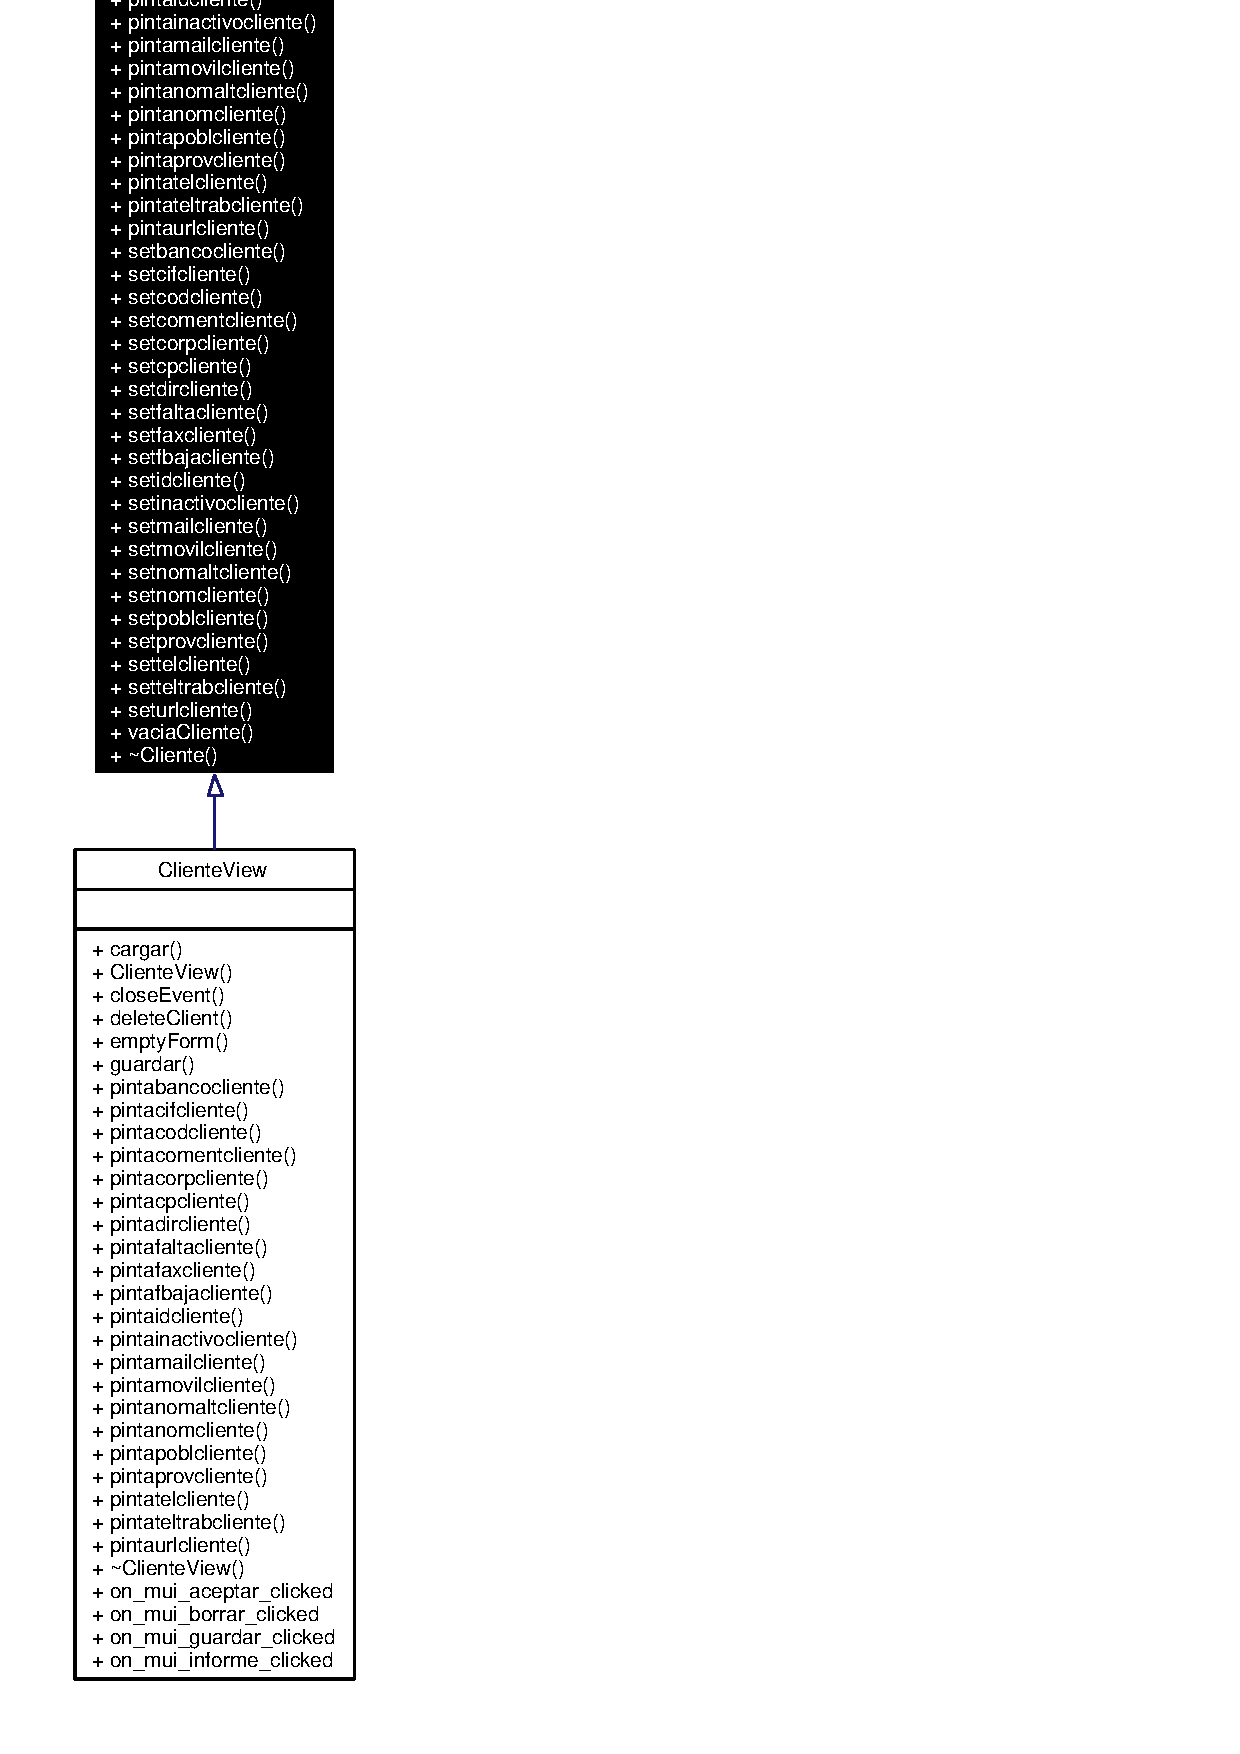
\includegraphics[width=85pt]{classCliente__inherit__graph}
\end{center}
\end{figure}
Diagrama de colaboraci\'{o}n para Cliente:\begin{figure}[H]
\begin{center}
\leavevmode
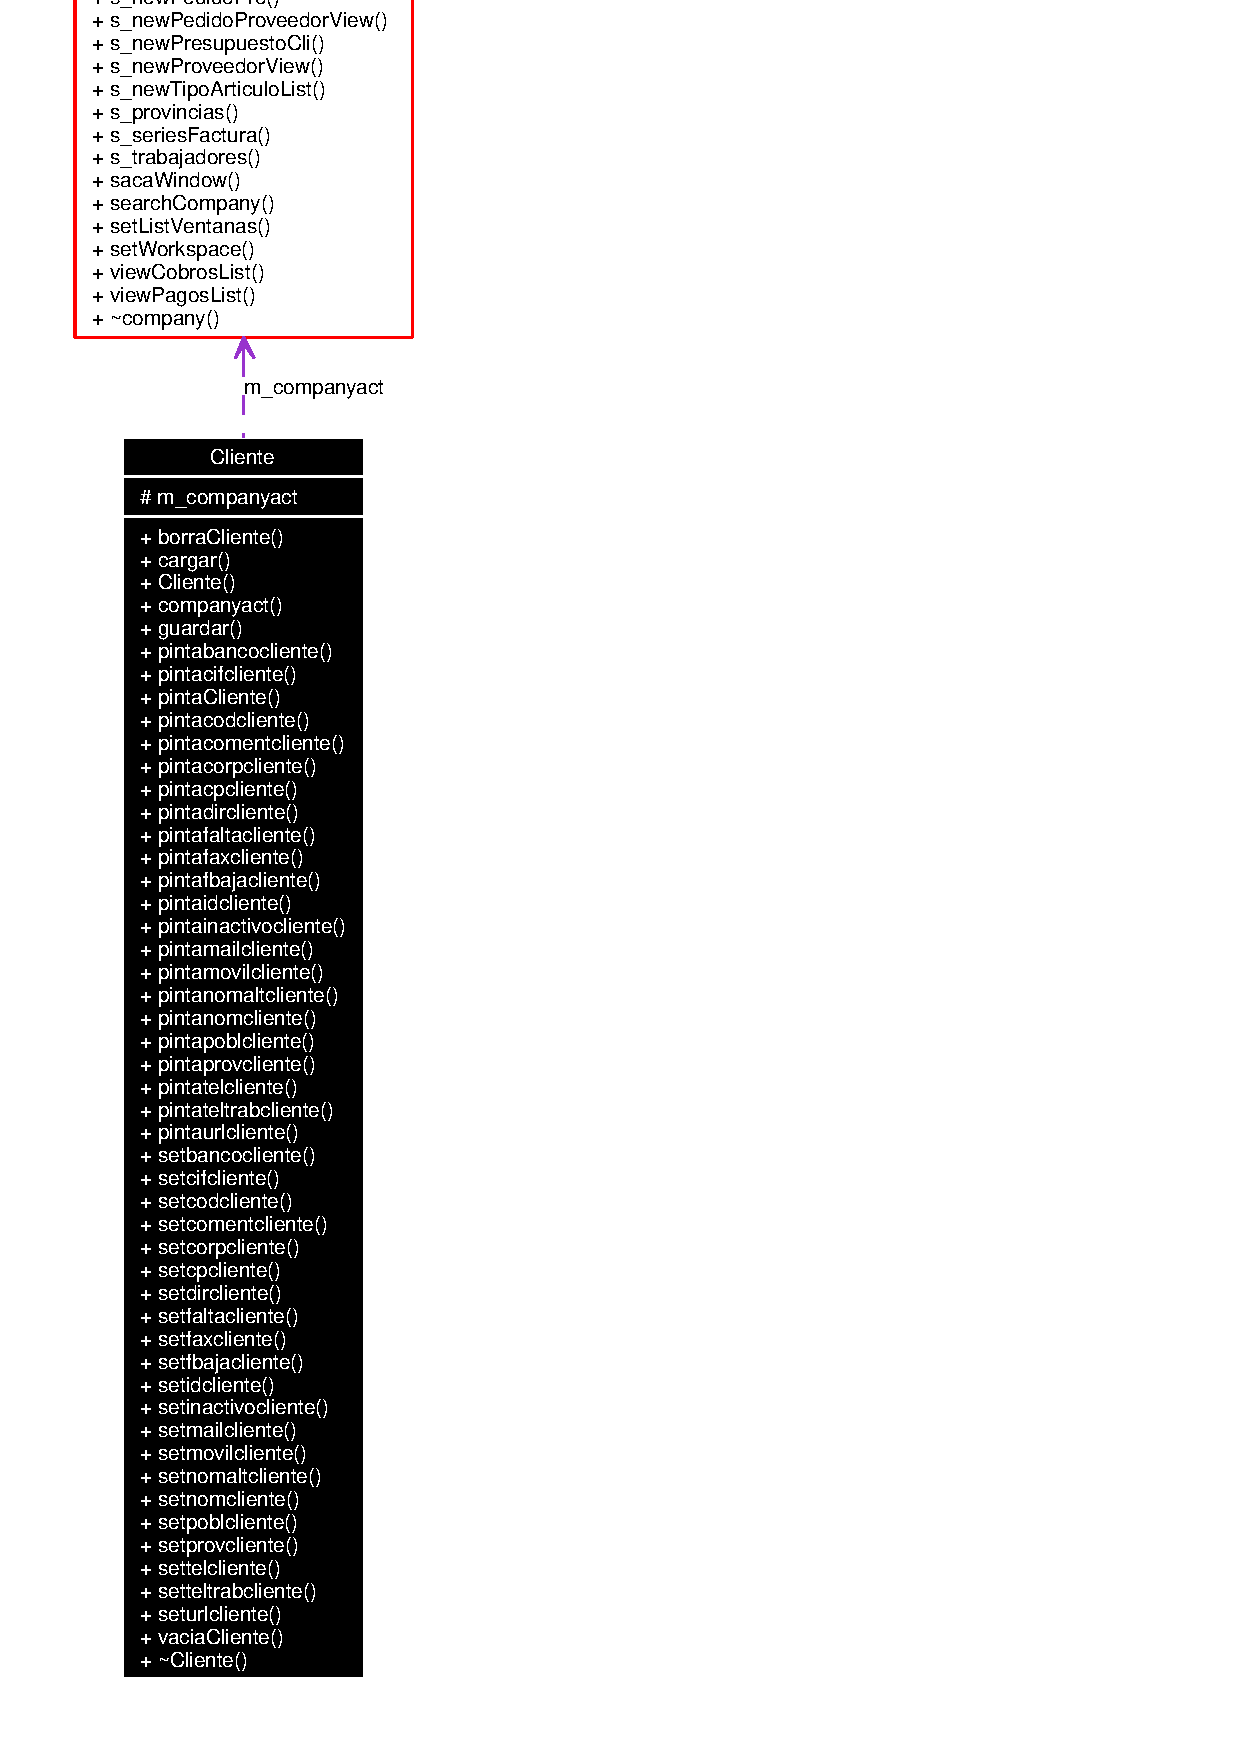
\includegraphics[width=99pt]{classCliente__coll__graph}
\end{center}
\end{figure}
\subsection*{M\'{e}todos p\'{u}blicos}
\begin{CompactItemize}
\item 
virtual void {\bf borra\-Cliente} ()\label{classCliente_a0}

\item 
virtual int {\bf cargar} (QString)\label{classCliente_a1}

\begin{CompactList}\small\item\em Esta funcion carga un cliente. \item\end{CompactList}\item 
{\bf Cliente} ({\bf company} $\ast$)\label{classCliente_a2}

\item 
{\bf company} $\ast$ {\bf companyact} ()\label{classCliente_a3}

\item 
virtual int {\bf guardar} ()\label{classCliente_a4}

\item 
virtual void {\bf pintabancocliente} (QString)\label{classCliente_a5}

\item 
virtual void {\bf pintacifcliente} (QString)\label{classCliente_a6}

\item 
virtual void {\bf pinta\-Cliente} ()
\item 
virtual void {\bf pintacodcliente} (QString)\label{classCliente_a8}

\item 
virtual void {\bf pintacomentcliente} (QString)\label{classCliente_a9}

\item 
virtual void {\bf pintacorpcliente} (QString)\label{classCliente_a10}

\item 
virtual void {\bf pintacpcliente} (QString)\label{classCliente_a11}

\item 
virtual void {\bf pintadircliente} (QString)\label{classCliente_a12}

\item 
virtual void {\bf pintafaltacliente} (QString)\label{classCliente_a13}

\item 
virtual void {\bf pintafaxcliente} (QString)\label{classCliente_a14}

\item 
virtual void {\bf pintafbajacliente} (QString)\label{classCliente_a15}

\item 
virtual void {\bf pintaidcliente} (QString)\label{classCliente_a16}

\item 
virtual void {\bf pintainactivocliente} (QString)\label{classCliente_a17}

\item 
virtual void {\bf pintamailcliente} (QString)\label{classCliente_a18}

\item 
virtual void {\bf pintamovilcliente} (QString)\label{classCliente_a19}

\item 
virtual void {\bf pintanomaltcliente} (QString)\label{classCliente_a20}

\item 
virtual void {\bf pintanomcliente} (QString)\label{classCliente_a21}

\item 
virtual void {\bf pintapoblcliente} (QString)\label{classCliente_a22}

\item 
virtual void {\bf pintaprovcliente} (QString)\label{classCliente_a23}

\item 
virtual void {\bf pintatelcliente} (QString)\label{classCliente_a24}

\item 
virtual void {\bf pintateltrabcliente} (QString)\label{classCliente_a25}

\item 
virtual void {\bf pintaurlcliente} (QString)\label{classCliente_a26}

\item 
void {\bf setbancocliente} (QString val)\label{classCliente_a27}

\item 
void {\bf setcifcliente} (QString val)\label{classCliente_a28}

\item 
void {\bf setcodcliente} (QString val)\label{classCliente_a29}

\item 
void {\bf setcomentcliente} (QString val)\label{classCliente_a30}

\item 
void {\bf setcorpcliente} (QString val)\label{classCliente_a31}

\item 
void {\bf setcpcliente} (QString val)\label{classCliente_a32}

\item 
void {\bf setdircliente} (QString val)\label{classCliente_a33}

\item 
void {\bf setfaltacliente} (QString val)\label{classCliente_a34}

\item 
void {\bf setfaxcliente} (QString val)\label{classCliente_a35}

\item 
void {\bf setfbajacliente} (QString val)\label{classCliente_a36}

\item 
void {\bf setidcliente} (QString val)\label{classCliente_a37}

\item 
void {\bf setinactivocliente} (QString val)\label{classCliente_a38}

\item 
void {\bf setmailcliente} (QString val)\label{classCliente_a39}

\item 
void {\bf setmovilcliente} (QString val)\label{classCliente_a40}

\item 
void {\bf setnomaltcliente} (QString val)\label{classCliente_a41}

\item 
void {\bf setnomcliente} (QString val)\label{classCliente_a42}

\item 
void {\bf setpoblcliente} (QString val)\label{classCliente_a43}

\item 
void {\bf setprovcliente} (QString val)\label{classCliente_a44}

\item 
void {\bf settelcliente} (QString val)\label{classCliente_a45}

\item 
void {\bf setteltrabcliente} (QString val)\label{classCliente_a46}

\item 
void {\bf seturlcliente} (QString val)\label{classCliente_a47}

\item 
virtual void {\bf vacia\-Cliente} ()\label{classCliente_a48}

\end{CompactItemize}
\subsection*{Atributos protegidos}
\begin{CompactItemize}
\item 
{\bf company} $\ast$ {\bf m\_\-companyact}\label{classCliente_p0}

\end{CompactItemize}


\subsection{Descripci\'{o}n detallada}
Administra los datos de un cliente. 



\subsection{Documentaci\'{o}n de las funciones miembro}
\index{Cliente@{Cliente}!pintaCliente@{pintaCliente}}
\index{pintaCliente@{pintaCliente}!Cliente@{Cliente}}
\subsubsection{\setlength{\rightskip}{0pt plus 5cm}void Cliente::pinta\-Cliente ()\hspace{0.3cm}{\tt  [virtual]}}\label{classCliente_a7}


Disparamos los plugins con presupuesto\_\-imprimir\-Presupuesto. 

La documentaci\'{o}n para esta clase fu\'{e} generada a partir de los siguientes archivos:\begin{CompactItemize}
\item 
cliente.h\item 
cliente.cpp\end{CompactItemize}
